%----------------------------------------------------------------------------------------
%	PACKAGES AND THEMES
%----------------------------------------------------------------------------------------
\documentclass[aspectratio=169,xcolor=dvipsnames]{beamer}
\usetheme{Simple}

\usepackage{graphicx} % Allows including noisy
\usepackage{booktabs} % Allows the use of \toprule, \midrule and \bottomrule in tables
\usepackage{hyperref}

% begin BibLaTeX section
\usepackage[backend=biber,texencoding=utf8,bibencoding=utf8,style=ieee,maxnames=3,bibwarn=true]{biblatex}
%\renewcommand*{\revsdnamepunct}{} % to eliminate the extra comma between last name and firstmiddle initials
% remember to include the *.bib extension on filenames in the \addbibresource{BibliographicResourceFile} command
\addbibresource{Denoising.bib}
\AtEveryBibitem{\clearlist{language}} % removes unnecessary use of "eng" as language
\AtBeginBibliography{\small}
% end BibLaTeX section
\renewcommand{\vec}[1]{\mathbf{#1}}
%----------------------------------------------------------------------------------------
%	TITLE PAGE
%----------------------------------------------------------------------------------------

% The title
\title[Denoising with SVD]{Image Denoising via Low-Rank Approximation\\ and Optimal Hard Thresholding}
\subtitle{MAT 167 - Applied Linear Algebra}

\author[Taswell and Garg] {Koby Taswell and Ayush Garg}
\institute[UCD] % Your institution may be shorthand to save space
{
	% Your institution for the title pag
	University of California, Davis 
	\vskip 3pt
}
\date{\today} % Date, can be changed to a custom date


%----------------------------------------------------------------------------------------
%	PRESENTATION SLIDES
%----------------------------------------------------------------------------------------

\begin{document}
	
	\begin{frame}
		% Print the title page as the first slide
		\titlepage
	\end{frame}
	
	\begin{frame}{Overview}
		% Throughout your presentation, if you choose to use \section{} and \subsection{} commands, these will automatically be printed on this slide as an overview of your presentation
		\tableofcontents
	\end{frame}
	
	%------------------------------------------------
	\section{Theory}
	%------------------------------------------------
	
	\begin{frame}{Singular Value Decomposition}
		\begin{itemize}
			\item Suppose we want to decompose a matrix with a method analogous to Eigenvalue decomposition, but applied to all matricies, not just square matricies \cite{Eckart1936}.
			\item \textbf{Singular value decomposition} provides ability to generalize from $A = \Phi\Lambda\Phi^{-1}$ to $A = U\Sigma V^{T}$
			\item For a given matrix $A$ which is size $m\times n$, $U$ is the left unitary matrix forming an orthonormal basis for $\mathbb{R}^m$  while $V$ is the right unitary matrix forming an orthonormal basis for $\mathbb{R}^n$
			\item $\Sigma$ is an $m\times n$ diagonal matrix of the singular values where $\sigma_1 \geq \sigma_2 \geq \sigma_n$. 
			\item Each combination of of $\vec{u}_i$, $\sigma_i$, and $\vec{v}_i$ for $1\leq i \leq \text{rank}(\Sigma)$ creates a rank one matrix $A_i = \sigma_i\vec{u}_i\vec{v}_i$.
			\item We can then approximate the original matrix $A$ by performing a \textbf{low rank approximation} of rank $k$ with $A_k = \sum_{i=1}^{k}  \sigma_i\vec{u}_i\vec{v}_i$
		\end{itemize}
	\end{frame}
	
	%------------------------------------------------
	
	\begin{frame}{Low Rank Approximation}
		\begin{itemize}
			\item One way to look at singular values is the amount that a specific pair of $\vec{u}_i, \vec{v}_i$ contributes to the reconstruction of $A$.
			\item We know from properties of the SVD, that the number of singular values in $\Sigma$ is the rank of the matrix.
			\item Suppose we have a matrix $A$ that is not full rank. A sufficient low rank approximation, would be to \textbf{truncate} $U$ and $V$ to only use a number of columns equal to the rank of our matrix. Then $A = \hat{U}\hat{\Sigma}\hat{V}^T = \sum_{i=1}^{r} \sigma_i\vec{u}_i\vec{v}_i^T$. 
			\item This let's us use less data to store the same or approximately similar information for $A$.
			\item So, what if we want to use even less space to store the same or approximately similar information?
			\item Additionally, what if we have some undesired variation of information called \textbf{noise} within the dataset, can we remove this unnecessary data by doing a low rank approximation?
		\end{itemize}
	\end{frame}
	%------------------------------------------------
	
	\begin{frame}{Thresholding}
		\begin{itemize}
			\item In essence, we want to find an approximation where if a singular value does not contribute enough to the matrix $A$, we disregard it.
	\begin{block}{Note}
		To simplify notation and reduce confusion we will refer to singular values as $y$ and noise level as $\sigma$ going forward
	\end{block}
			\item How can we determine this?
			\item Choose a threshold $\tau$, if a singular value $\sigma_i$ is below our threshold ($y_i < \tau$), then set $y_i=0$
			\item In doing so, we find an estimation of $A$ which uses less data and is of lower rank. For the values of $y_i = 0$, the corresponding $\vec{u}_i\vec{v}_i$
			\item In general we can choose $\tau = \lambda\sqrt{n}\sigma$\cite{Chatterjee2015} where $n$ is the size of a square matrix and $\lambda$ is some coefficient typically between 1 and 10.
		\end{itemize}
	\end{frame}
	
	%------------------------------------------------
	
	\begin{frame}{Finding our Threshold $\tau$ based on $\lambda$}
		\begin{itemize}
			\item Bulk Edge Thresholding which excludes any singular values below the 'gap' or 'elbow' when plotted. $\lambda = (1+\sqrt{\beta})$ where $\beta = \frac{m}{n}$.
			\item Chatterjee proposed that there exists some $\lambda$ regardless of rank or shape of matrix which would give a near optimal mean square error between the original matrix $A$ and the reconstructed low rank approximation. In his paper, Chatterjee suggested $\lambda \approx 2.02$ \cite{Chatterjee2015}.  
			\item In 2013, Gavish \& Donoho defined two methods:
			\begin{enumerate}
				\item For an arbitrary $m\times n$ matrix where $\sigma$ is unknown: $\tau = 2.858y_{\text{med}}$ and $y_{\text{med}}$ is the median of the singular values.
				\item For a square $m\times n$ matrix where $\sigma$ is known: $\tau = \lambda_\beta\sqrt{n}\sigma$ 
			\end{enumerate}
			\begin{itemize}
				\item When matrix is $n\times n$, $\beta = 1$ and they define the optimal $\lambda_\beta = \frac{4}{\sqrt{3}}\approx 2.3094$
				\item When matrix is $m\times n$, $\beta \neq 1$, use different $\lambda_\beta$ see paper for more\cite{Gavish2013}
			\end{itemize}
		\end{itemize}
	\end{frame}
	
	%------------------------------------------------
	\section{Simple Example - Kingfisher}
	%------------------------------------------------
	
	\begin{frame}{Simple Example - Kingfisher}
		\centering
		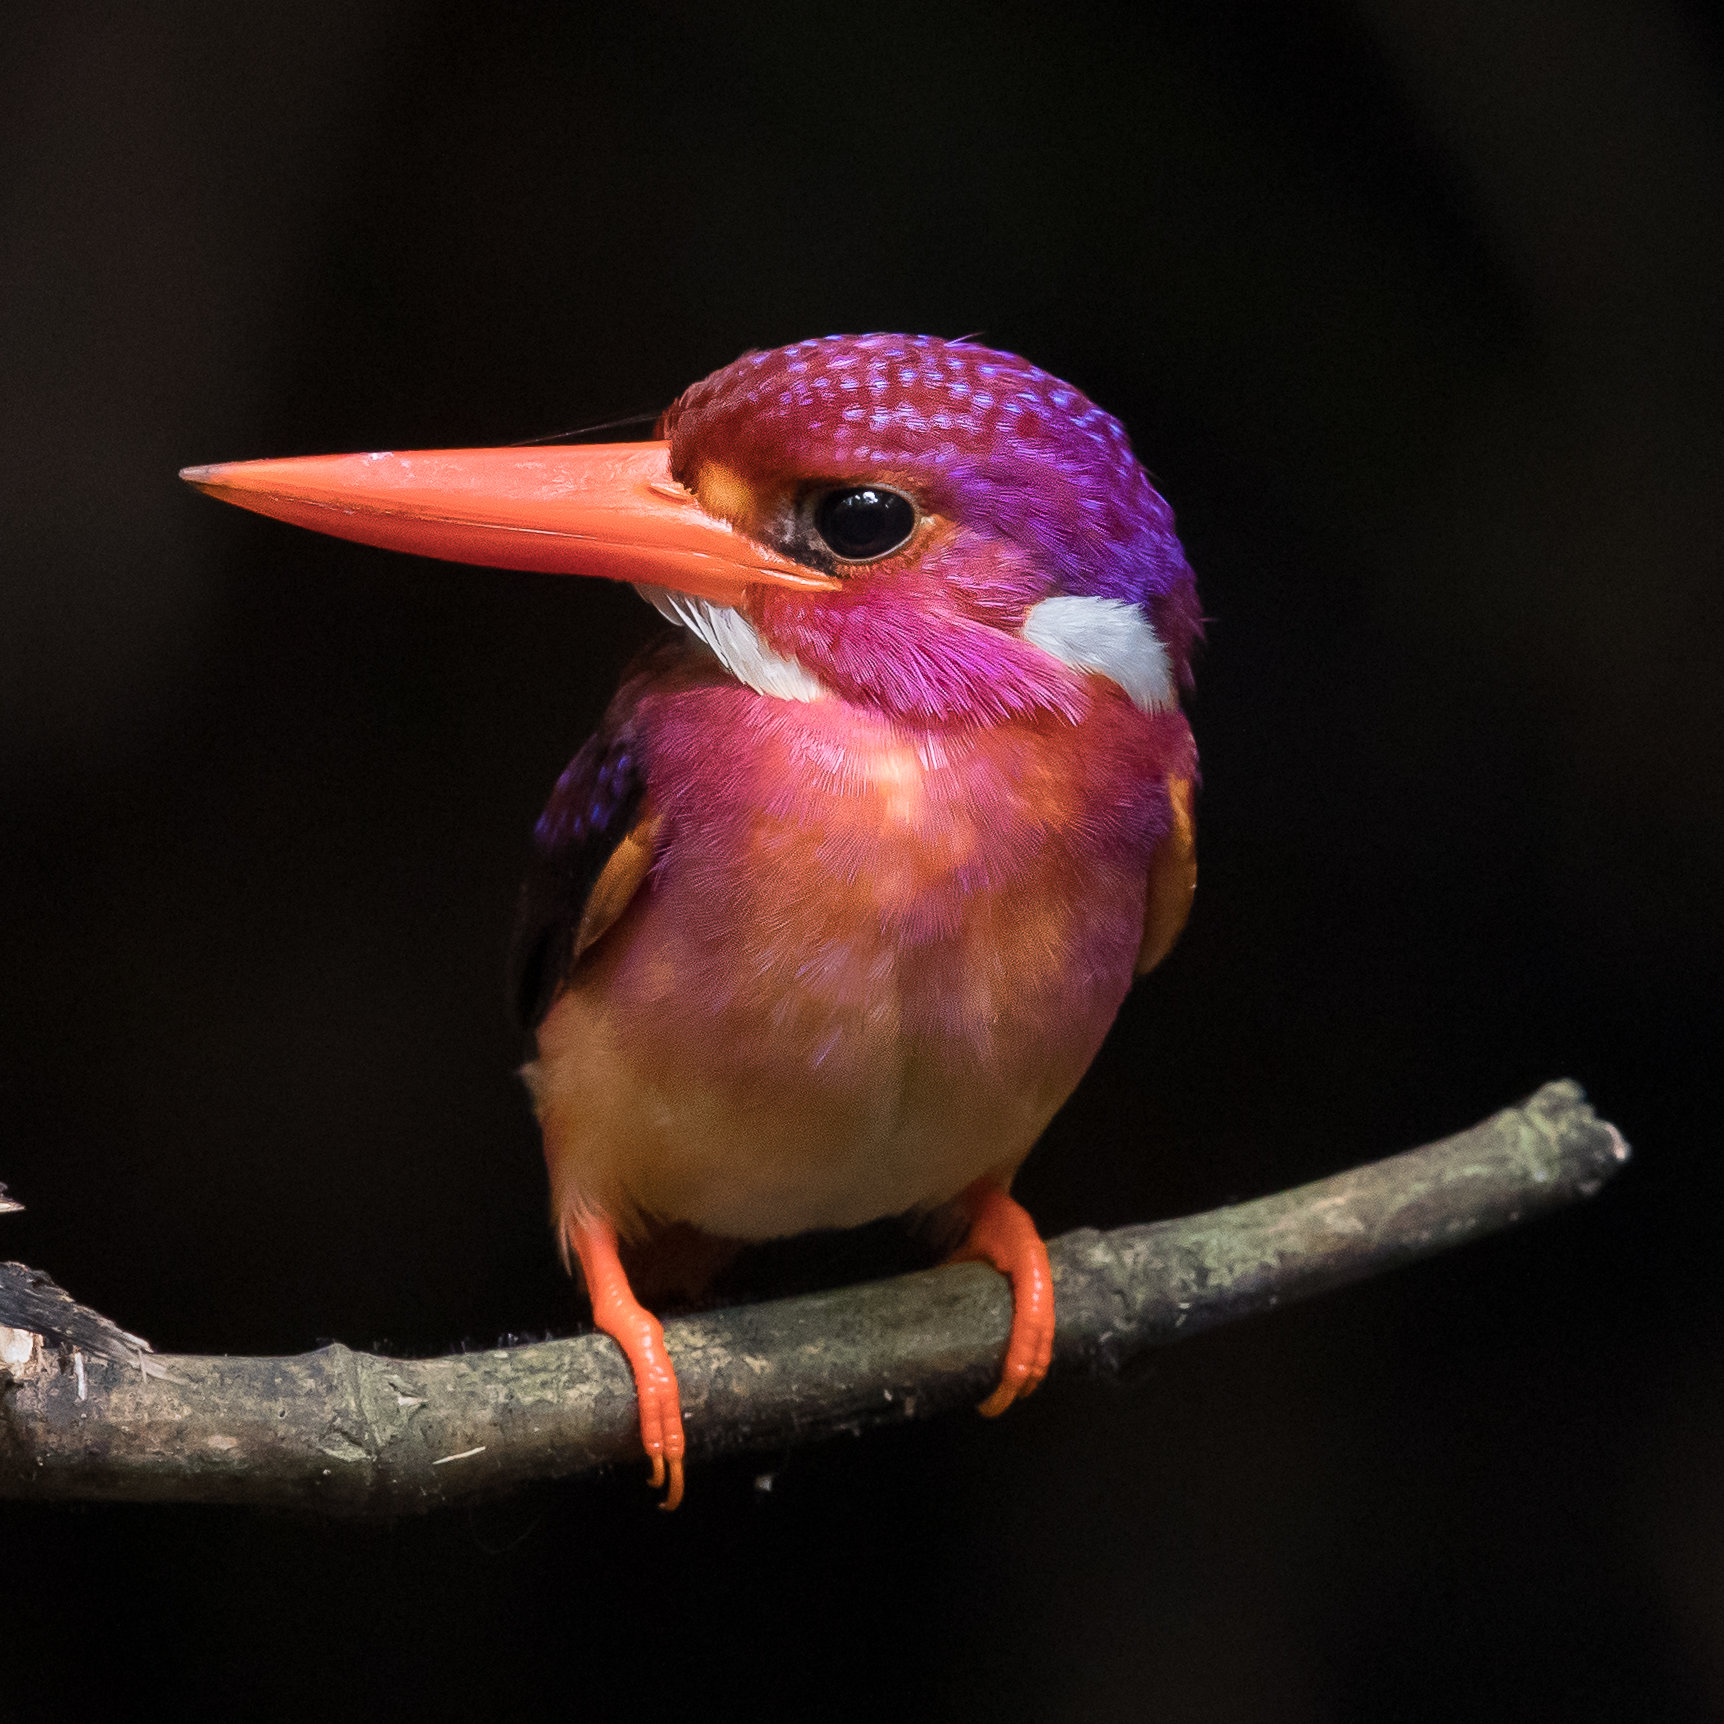
\includegraphics[scale=0.5]{Kingfisher.jpg}
	\end{frame}

	%------------------------------------------------

	\begin{frame}[fragile]{A Noisy Image}
		\begin{itemize}
			\item Suppose we have noise in an image. We can simulate this by adding noise to our beautiful picture of a Kingfisher in MATLAB with \verb*|imnoise(I)|	
			\item Image Properties: $1724\times1724$ in full JPG RGB color scale from 0 to 255 for Red, Green, and Blue.
		\end{itemize}
		\begin{figure}
			\centering
			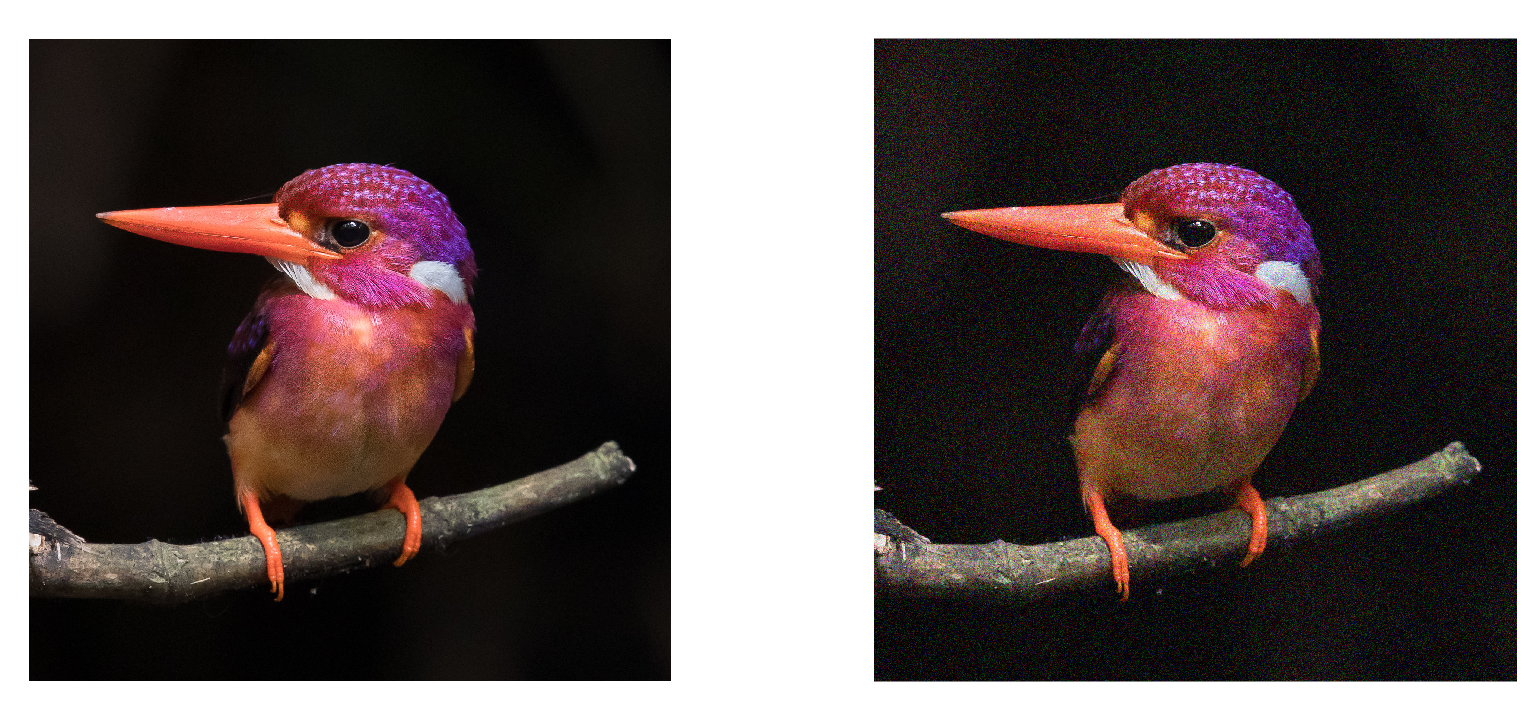
\includegraphics[scale=0.35]{KingfisherWNoise.png}
		\end{figure}
	\end{frame}
	
	%------------------------------------------------
	
	\begin{frame}{Measuring Noise in an Image}
		\begin{itemize}
			\item \textbf{Mean Squared Error:} Measure the average difference between two matricies by performing $\text{MSE} = \frac{1}{mn}\sum_{i=1}^m\sum_{j=1}^{n}(a_{ij}-\hat{a}_{ij})^2$
			\item \textbf{Frobenius Norm:} Calculate $\|A-\hat{A}\|_F$ to find the 'distance' between the two matricies\cite{Shabalin2013}.  
			\item \textbf{Signal-Noise Ratio:} In general $\text{SNR} = \frac{P_{signal}}{P_{noise}}$ where $P$ refers to the power of the signal or noise. More specifically this could be $\text{SNR} = \frac{s^2}{EN^2}$ where $E$ is the expected value and $N$ is the random noise.
		\end{itemize}
	\begin{figure}
		\centering
		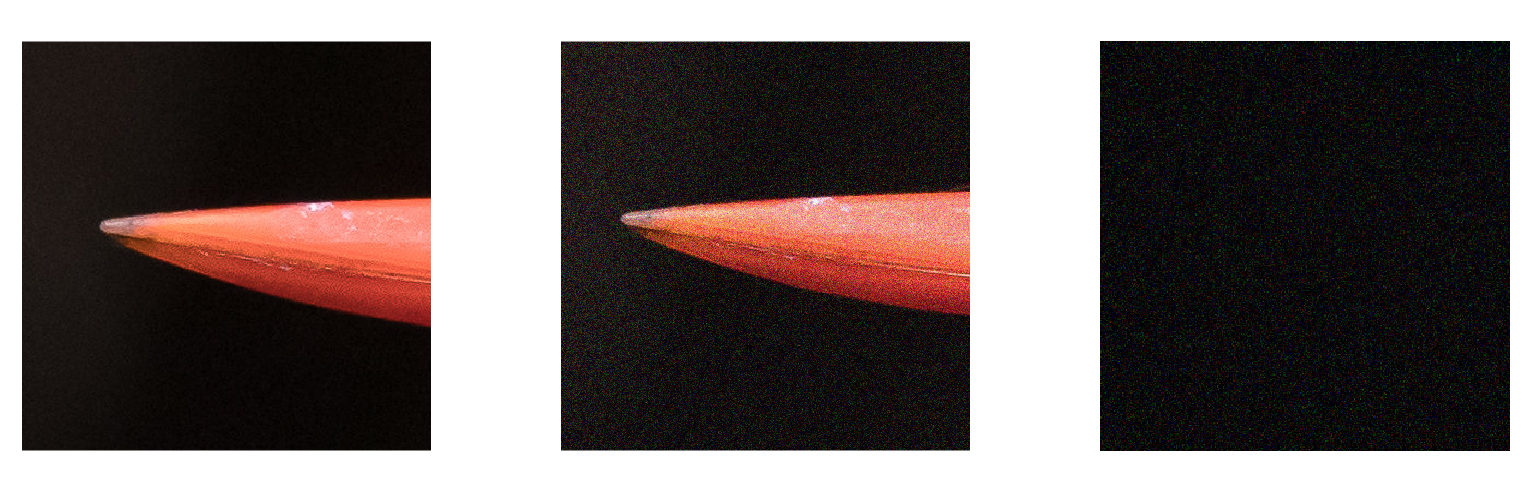
\includegraphics[scale=0.3]{BeakNoise.png}
		\caption{Comparison of Zoomed in Beak between Original, Noisy, and Noise only Images}
	\end{figure}
	\end{frame}
	
	%------------------------------------------------
	
	\begin{frame}{Removing Noise with Arbitrary Thresholding}
		\begin{itemize}
			\item Methods for Arbitrary Thresholding: 
			\begin{enumerate}
				\item Calculate SVD of Noisy Image for each color channel Red, Green, and Blue
				\item Find $y_{\text{med}}$
				\item Apply threshold $\tau = 2.858y_{\text{med}}$
				\item Find $\hat{A} = \hat{U}\hat{\Sigma}\hat{V}^T$
			\end{enumerate}
		\end{itemize}
		\begin{figure}
		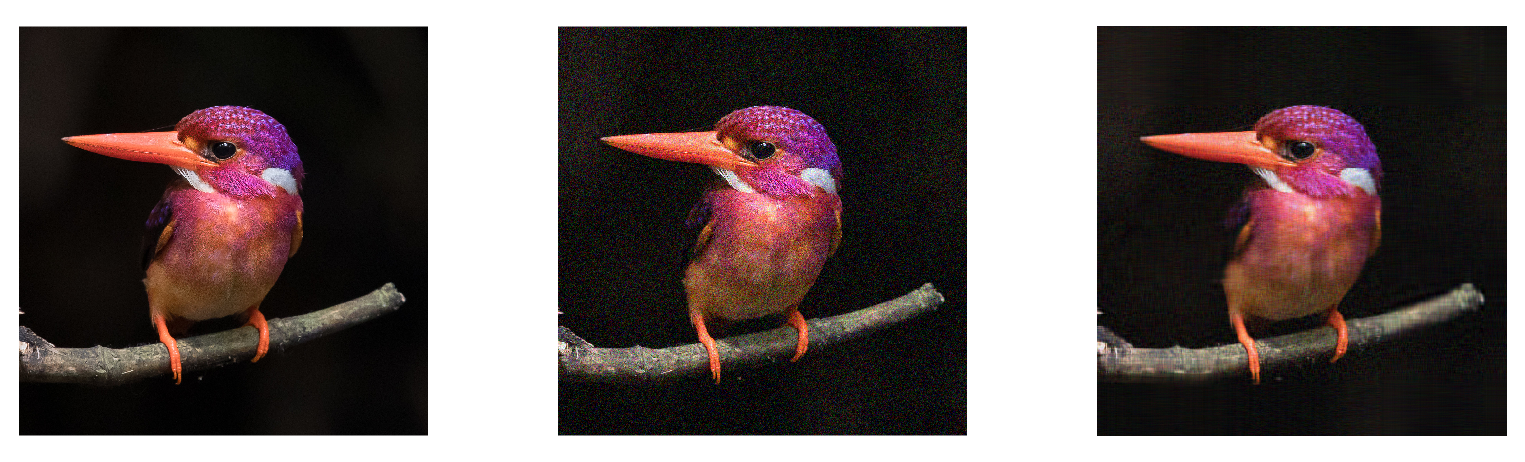
\includegraphics[scale=0.4]{ArbitraryDenoise.png}
		\caption{Comparison of Original, Noisy, and Arbitrary Threshold Denoised Images}
		\end{figure}
	\end{frame}
	
	%------------------------------------------------
	
	\begin{frame}{Removing Noise with Non-arbitrary Thresholding}
		\begin{itemize}
			\item Methods for Non-arbitrary Thresholding: 
			\begin{enumerate}
				\item Calculate SVD of Noisy Image for each color channel Red, Green, and Blue
				\item Find signal to noise ratio $\sigma$
				\item Since the image is $n\times n$, Apply threshold $\tau = \frac{4}{\sqrt{3}}\sqrt{n}\sigma$
				\item Find $\hat{A} = \hat{U}\hat{\Sigma}\hat{V}^T$
			\end{enumerate}
		\end{itemize}
		\begin{figure}
			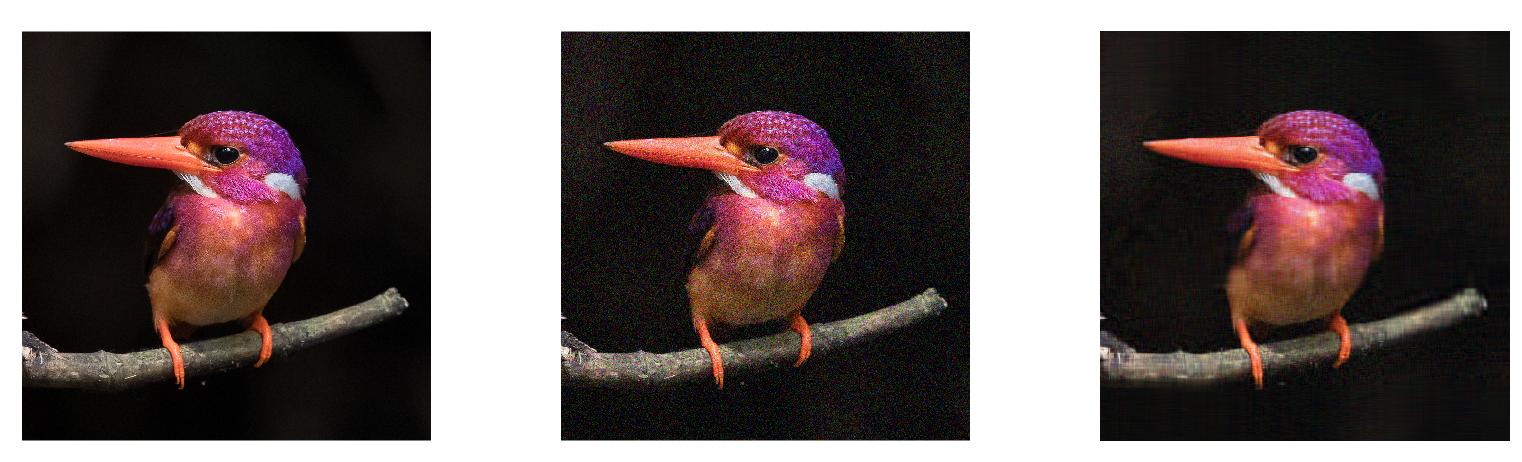
\includegraphics[scale=0.4]{SquareDenoise.png}
			\caption{Comparison of Original, Noisy, and Non-arbitrary Threshold Denoised Images}
		\end{figure}
	\end{frame}
	
	%------------------------------------------------
	
	\begin{frame}{Removing Noise with Bulk Edge Thresholding}
		\begin{itemize}
			\item Methods for Bulk Edge Thresholding: 
			\begin{enumerate}
				\item Calculate SVD of Noisy Image for each color channel Red, Green, and Blue
				\item Find $\beta = \frac{m}{n}$
				\item Apply threshold $\tau = (1+\sqrt{\beta})\sqrt{n}\sigma$
				\item Find $\hat{A} = \hat{U}\hat{\Sigma}\hat{V}^T$
			\end{enumerate}
		\end{itemize}
		\begin{figure}
			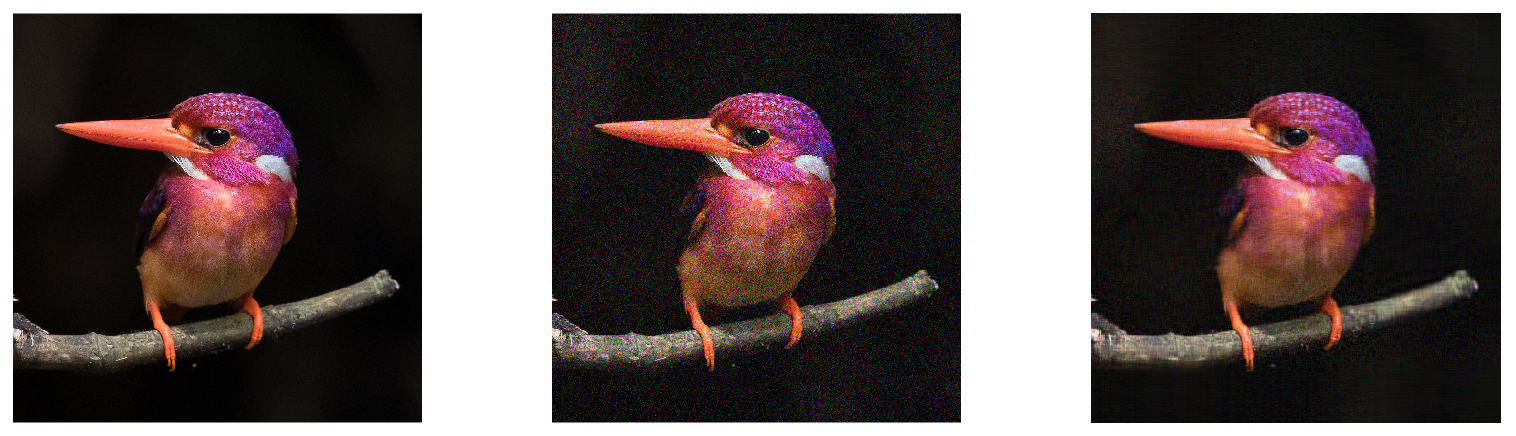
\includegraphics[scale=0.4]{BulkDenoise.png}
			\caption{Comparison of Original, Noisy, and Bulk Edge Threshold Denoised Images}
		\end{figure}
	\end{frame}
	
	%------------------------------------------------
	
	\begin{frame}{Performance}
		\begin{itemize}
			\item A keen eye might notice that there does \textbf{not} appear to be a large amount of difference between the results of our three thresholding methods.
			\item By evaluating original MSE of the raw image in comparison to the noisy image we find $\text{MSE}(I, I_{noisy}) = 0.0066$, a small but not insignificant amount of variance.
			\item When calculating the MSE of the raw image in comparison to all three of the denoised images, we find the exact same value $\text{MSE}(I, I_{denoised}) = 0.0022$ for an overall reduction of variance by 60\%. 
			\item However none of the three methods, despite having slightly different threshold values, had significant difference in results.
		\end{itemize}
	\end{frame}
	
	%------------------------------------------------
	
	\begin{frame}{Performance}
		\begin{itemize}
			\item A keen eye might notice that there does \textbf{not} appear to be a large amount of difference between the results of our three thresholding methods.
			\item By evaluating original MSE of the raw image in comparison to the noisy image we find $\text{MSE}(I, I_{noisy}) = 0.0066$, a small but not insignificant amount of variance.
			\item When calculating the MSE of the raw image in comparison to all three of the denoised images, we find the exact same value $\text{MSE}(I, I_{denoised}) = 0.0022$ meaning that approximately 2/3rds of the variance or noise in the image remained. 
			\item However none of the three methods, despite having slightly different threshold values, had significant difference in results.
			\item Another important note is that in losing a lot of noise, we've also lost some amount of signal (See pixelation on the branch and elsewhere). This is less noticeable since our image is already high resolution aka the matrix is large but will be easily noticeable in images that begin with significantly lower resolution.
		\end{itemize}
	\end{frame}

	%------------------------------------------------
	
	\begin{frame}{Results}
		\begin{table}
			\begin{tabular}{l | l | l | l |l}
				\toprule
				\textbf{Method} & \textbf{MSE} & \textbf{Frobenius} & \textbf{Signal to Noise (Db)} & \textbf{Approximation Rank k} \\
				\midrule
				Arbitrary          & 0.0022           & 79.963 &  $r_{red} = 15.5806$ &  $k_{red} = 54$ \\
				& & & $r_{green} = 12.3801$ & $k_{green} = 45$ \\
				& & & $r_{blue} = 11.7773$ & $k_{blue} = 56$\\\hline
				Non-Arbitrary         & 0.0022            & 80.781 & $r_{red} = 15.3444$ & $k_{red} = 33$             \\
				& & & $r_{green} = 12.3539$ & $k_{green} = 41$\\
				& & & $r_{blue} = 11.7583$ & $k_{blue} = 41$\\\hline
				Bulk Edge       & 0.0022            & 81.282 & $r_{red} = 15.5387$ &      $k_{red} = 44$         \\
				& & & $r_{green} = 12.1211$ & $k_{green} = 71$\\
				& & & $r_{blue} = 11.6600$  & $k_{blue} = 75$\\
				\bottomrule
			\end{tabular}
			\caption{Comparison of results when denoising and approximating $r = 1724$ Red, Green, and Blue color matricies}
		\end{table}
	\end{frame}
	
	%------------------------------------------------
	\section{Hard Application - Medical Imaging}
	%------------------------------------------------
	
	\begin{frame}{References}
		% Beamer does not support BibTeX so references must be inserted manually as below
		\printbibliography
	\end{frame}
	
	%------------------------------------------------
	
	\begin{frame}
		\Huge{\centerline{The End}}
	\end{frame}
	
	%----------------------------------------------------------------------------------------
	
\end{document}